% -*- mode:LaTeX; mode:visual-line; mode:flyspell; fill-column:75 -*-
\section{Experiments and Results}
\label{sec:results}

We now present proof-of-concept experiments on a robot reaching task.
These early results serve as an initial demonstration of our ability to learn the correct behavior from user demonstrations and apply those when the user provides natural language command during task execution.

The robot is tasked with reaching a goal, and the initial Dynamical System is a linear dynamics model with a stable attractor at the goal position; this results in straight-line trajectories towards the goal.
While this initial behavior correctly specifies the task (the \emph{what}), changes in the environment (such as the addition of a bin) may result in the robot incorrectly performing the task, as shown in \Cref{figBucket}. Note that in our experiments the robot has no sensors to detect obstacles.
Using natural language, the user can help the robot complete the task correctly by describing \emph{how} it should approach the goal position (in this case, ``come from above'').


\begin{figure}[t]
  \centering
  %% 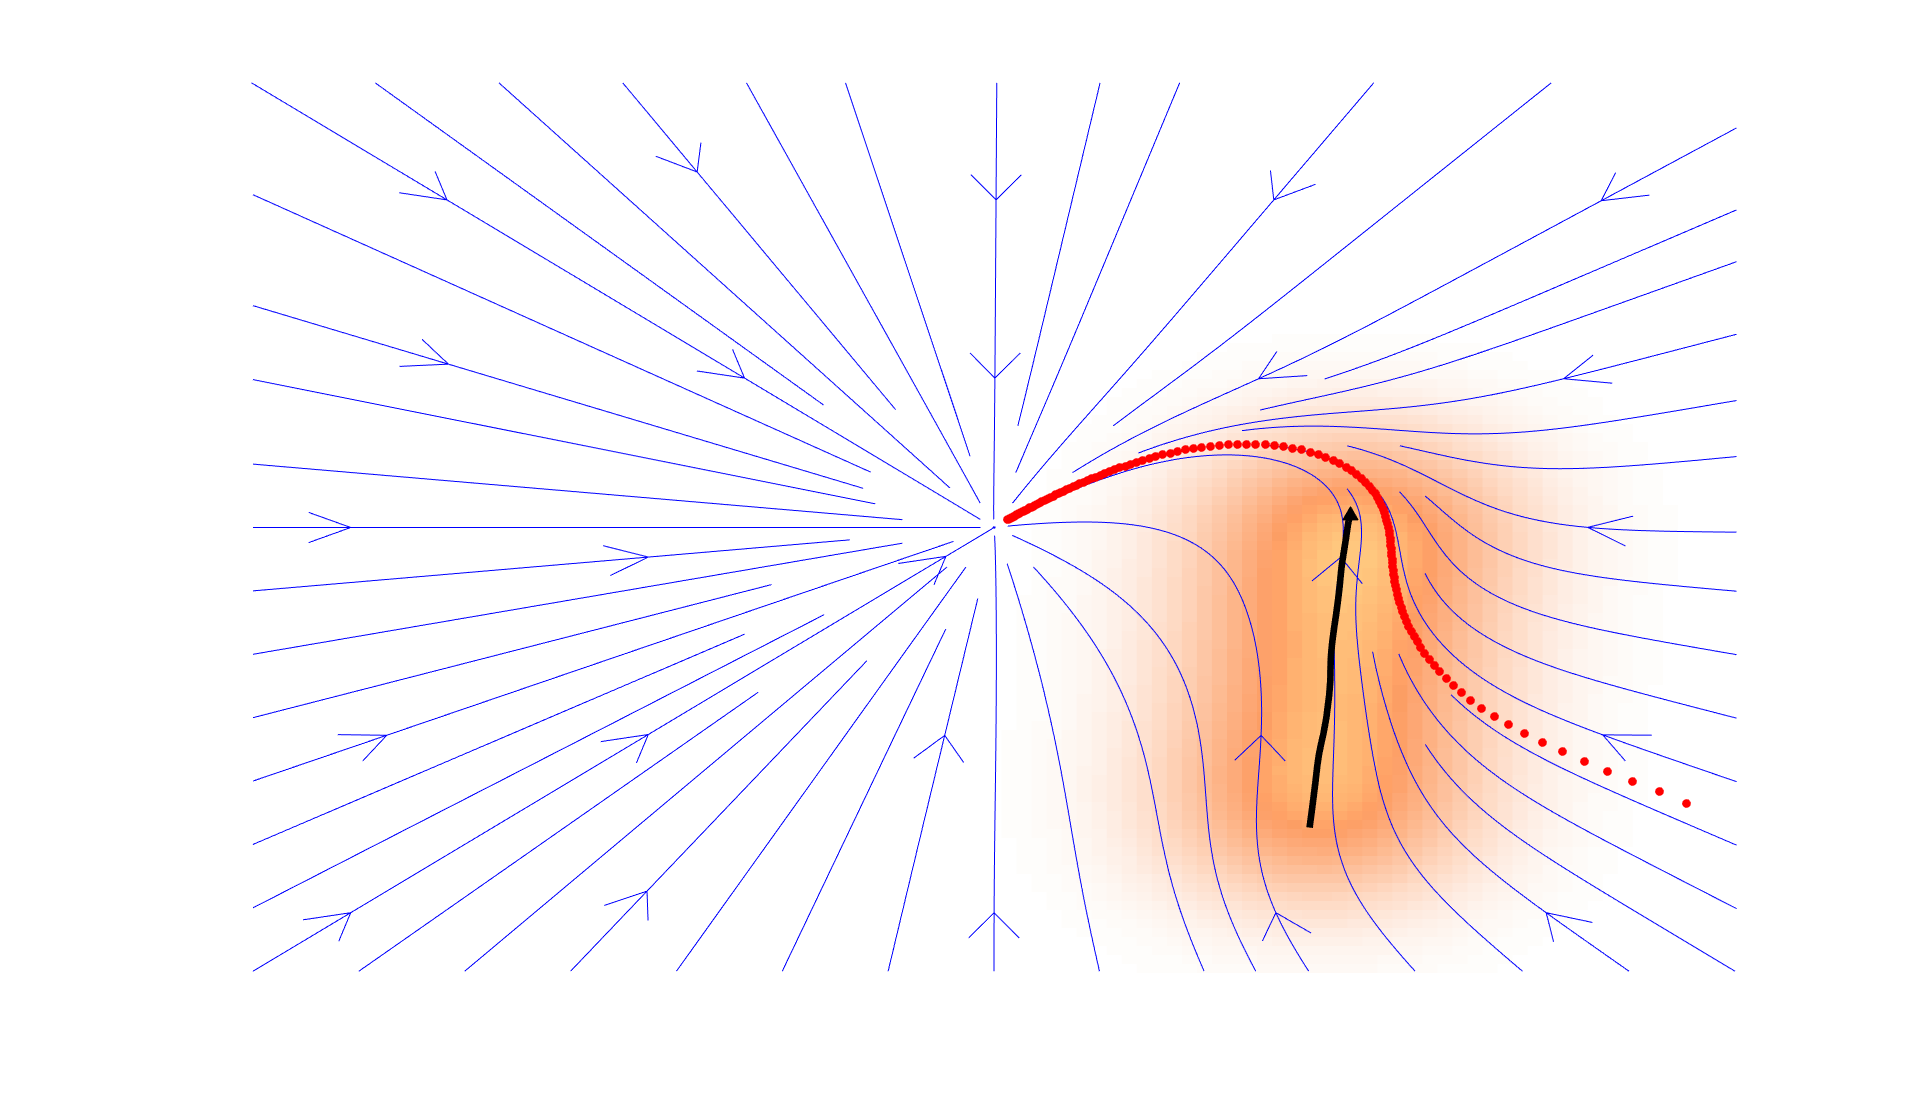
\includegraphics[
  %%   % trim = left bottom right top
  %%   trim = 150mm 50mm 100mm 80mm, clip,
  %%   width = 0.4\textwidth,
  %% ]{figs/gp_figs/3a-traj1.png}
  \missingfigure{Photo of the bucket}
  \caption{
    A scenario where the robot is unaware of the bucket and must get help from the user to reach the goal.
  }
  \label{figBucket}
\end{figure}
